%%% LaTeX Template: Article/Thesis/etc. with colored headings and special fonts
%%%
%%% Source: http://www.howtotex.com/
% vim: set spell spelllang=es syntax=tex :

\documentclass[12pt]{article}
\usepackage{styles/apuntes-estilo}
\usepackage{fancyhdr,lastpage}
\usepackage{hyperref}
\usepackage[inline]{enumitem}
\usepackage{xurl}
\usepackage{upquote}

\newcommand{\cw}[1]{\texttt{\textcolor{blue}{#1}}}

\newcommand{\bash}{\textbf{\texttt{BASH}}}

\def\maketitle{

\makeatletter{
    \color{blue} \centering \huge \sc
    \textbf{
        Trabajo práctico de Laboratorio 01\\
        \large \vspace*{-8pt} \color{black}
        Introducción al shell del sistema GNU/LINUX
        \vspace*{8pt}
    }
    \par
}

\makeatother

\makeatletter
% vim: set spell spelllang=es syntax=tex :
 {\centering \small 
    Introducción a la computación\\
    Departamento de Ingeniería de Computadoras \\
    Facultad de Informática - Universidad Nacional del Comahue \\
    \vspace{20pt} }
\makeatother

\vspace{-2.5cm}
\mbox{\hspace{-1cm}\includegraphics[width=3cm,height=3cm]{logos/uncoma.pdf}\hspace{12cm}
    
\includegraphics[width=3cm,height=3cm]{logos/fai.pdf}}



}

% Custom headers and footers
\fancyhf{} % clear all header and footer fields
\fancypagestyle{plain}{\fancyhf{}}
\pagestyle{fancy}
\lhead{\footnotesize Trabajo práctico de Laboratorio 01 - Introducción al shell del sistema GNU/LINUX}
\rhead{\footnotesize \thepage\ }

\def\ti#1#2{\texttt{#1} & #2 \\ }

\begin{document}

\thispagestyle{empty}
\maketitle
\setlength{\parindent}{1pt}

\textbf{Lectura obligatoria:}

\vspace{-2\topsep}
\begin{itemize}

    \itemsep2pt \parskip0pt \parsep0pt

    \item Apunte del shell de Linux:
        \url{http://pedco.uncoma.edu.ar/mod/resource/view.php?id=207175}

    \item Apunte introductorio a \bash:
        \url{http://pedco.uncoma.edu.ar/mod/resource/view.php?id=244968}

    \item Linux Man Pages Online: \url{https://linux.die.net/man/}

\end{itemize}

A continuación, se realizarán una serie de ejercicios para los cuales
necesitará acceso a una computadora con el sistema operativo de tipo \cw{UNIX}
(como por ejemplo alguna distribución \cw{GNU/Linux}) y las siguientes
aplicaciones:

\vspace{-2\topsep}
\begin{itemize}

    \itemsep2pt \parskip0pt \parsep0pt

    \item   Intérprete de comandos \bash{} y demás utilidades que se encuentran
        en la mayoría de las distribuciones de Linux.

    \item   Un editor de texto en la interfaz de línea de comando o gráfica.

\end{itemize}

Para un tutorial sobre como realizar una conexión remota a los laboratorios de
la facultad, diríjase al anexo de la página \pageref{sec:anexoConexion}.

\section{Entrando en calor con el \emph{shell} \bash}

El sistema operativo controla diferentes procesos de una computadora. Uno de
ellos es el intérprete de comandos o \emph{shell}. Este es un programa que
permite al usuario interactuar con el Sistema Operativo. Permite iniciar
(ejecutar) otros programas así como también tiene comandos propios que no
necesitan de otros programas, como por ejemplo comandos para movernos en la
estructura de directorios. En este práctico, utilizaremos el intérprete
\bash\emph{(Bourne-Again SHell)}, muy popular en el mundo de Linux.

Dicho programa debe ser ejecutado en lo que llamamos Terminal o Consola, que
es otro programa que nos permite interactuar mediante el teclado (ingresar
caracteres) y ver los resultados de la ejecución de otros programas en la
pantalla. Al iniciar una consola o terminal de textos, automáticamente se
inicia el \emph{shell} \bash, que es con el que el usuario realmente
interactúa (más abajo se explica esto con un ejemplo).

\begin{enumerate}

    \item Ingrese remotamente a los laboratorios siguiendo alguna de las
        opciones plateadas en el tutorial del anexo de la página
        \pageref{sec:anexoConexion}.
        
    \item Una vez realizada la conexión, el \emph{shell} \bash{} en la
        terminal espera que se escriban órdenes para ejecutar (comandos). En
        la terminal escriba el comando \cw{hostname} y presione la tecla
        \emph{enter} para verificar el nombre del equipo al que se conecto.
        ¿Cuál es el nombre del equipo?

    \item Ejecute el comando \cw{who} para ver que usuarios están conectados
        actualmente al sistema ¿Cuántos usuarios están conectados actualmente?

    \item Ejecute \cw{last | tac} para ver la lista de últimas conexiones
        ¿Reconoce a alguno de los usuarios?

    \item Ejecute el comando \cw{lscpu} para ver las características del
        \emph{CPU} del sistema al que se ha conectado ¿Cuántos núcleos tiene
        el sistema?

    \item Ejecute el comando \cw{man free} para leer el manual del comando
        \cw{free}. Para salir, presione la tecla \cw{q}.

    \item Ejecute el comando \cw{free} ¿Cómo puede hacer para que muestre la
        información en \cw{GiB}? ¿Cuántos \cw{GiB} tiene el sistema?
        \emph{(ayuda: lea el manual)}

    \item Ejecute el comando \cw{top} para ver los procesos que están
        ejecutando en el sistema de forma dinámica, así como información del
        uso del tiempo de \emph{CPU} y memoria. Para salir, presione la tecla
        \cw{q}. Identifique la cantidad de memoria utilizada actualmente.

\end{enumerate}

\section{Sistemas de archivos}

\label{sec:sistemaDeArchivos}

El concepto de directorios (comúnmente llamados ``carpetas'') y archivos es
hoy en día familiar a los usuarios de computadoras. En general el usuario se
maneja visualmente con el ratón y el Explorador de Archivos, utilizando estos
para acceder a los directorios, abrir archivos, ejecutar programas, etc.
Podemos pensar el sistema de archivos como una forma de organizar todo el
contenido en el dispositivo de almacenamiento. Los archivos son datos
concretos, utilizan espacio físico del dispositivo, mientras que los
directorios sirven para organizar ``lógicamente'' las cosas, igual que una
persona tiene estanterías y cajones en un escritorio para organizar sus
papeles.

La figura \ref{arbolDirectorios}  muestra un esquema de como se puede pensar en
una estructura de directorios y archivos. \cw{ic}, \cw{parciales} y
\cw{imagenes} son directorios, mientras que \cw{notas.tsv}, \cw{p1.pdf},
\cw{p2.pdf} y \cw{gatito.jpg} son archivos.

\begin{figure}[!htb]

    \centering

    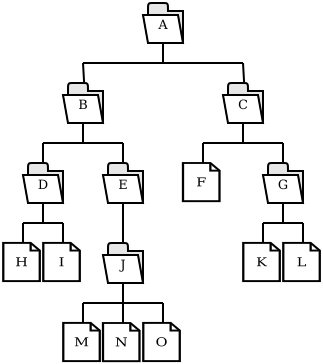
\includegraphics[height=0.45\textheight]{img/directorios.pdf}

    \caption{Árbol de directorios.}

    \label{arbolDirectorios}

\end{figure}

Cuando se inicia el intérprete de comandos, éste se posiciona en una
determinada carpeta, es decir, los comandos que se escriben afectarán
directamente al contenido de dicha carpeta.

En general, al iniciar una consola de texto, junto con un intérprete de
comandos, se posiciona al usuario en la carpeta personal o \textbf{``HOME''}
(en Linux en general es \cw{``/home/usuarioX''}). Desde aquí el usuario
puede navegar por sus archivos y ejecutar comandos. Para saber cual es el
directorio en el que se encuentra, ejecute el comando \cw{pwd} (\emph{Print
Working Directory}).

Además, existen dos formas de hacer referencia a los directorios y a los
archivos en el intérprete, absoluta y relativa. Cuando utilizamos la forma
absoluta se escribe todo el camino desde la carpeta inicial (en \cw{Linux}
se denota con el símbolo \cw{``/''}) hasta la ubicación deseada. Ejemplos de
uso absoluto: \cw{/home/usuario/trabajo1}, \cw{/etc}, \cw{/tmp}, etc.

El modo relativo sirve para hacer referencia a un directorio que se encuentra
``cerca'' del directorio de trabajo actual en la jerarquía, como por ejemplo
el directorio directamente superior o inferior.

Por ejemplo, las siguientes son direcciones relativas:

\vspace{-2\topsep}
\begin{itemize}

    \itemsep2pt \parskip0pt \parsep0pt

    \item \cw{./} (el directorio actual)

    \item \cw{../} (directorio inmediatamente superior)

    \item \cw{./trabajo1} (directorio \cw{trabajo1} ubicado dentro del
        directorio actual)

    \item \cw{../../archivoX} (archivo ubicado dos directorios más arriba en
        la jerarquía)

\end{itemize}

\begin{enumerate}[resume]

    \item Ejecute el comando \cw{pwd} para ver en que directorio se encuentra
        actualmente el shell.

    \item Ejecute el comando \cw{ls} para listar los archivos que se
        encuentran en el directorio actual.

    \item Para crear un archivo de texto ejecute el comando \cw{nano
        archivo.txt}. Escriba el texto que le plazca (puede ser un poema, una
        frase sabia, o \cw{ASCII Art}). Para guardar presione \emph{Ctrl+O},
        presione \emph{enter} para confirmar, y presione \emph{Ctrl+X} para
        salir.

    \item Ejecute el comando \cw{ls} para verificar que el archivo fue creado
        exitosamente.

    \item Ejecute el comando \cw{cat archivo.txt} para mostrar el contenido
        del archivo en pantalla.

    \item Para mayor dramatismo, ejecute lo siguiente: \cw{cat archivo.txt |
        cowsay -n | lolcat} ¿Qué hace cada uno de los comandos de la
        secuencia?

    \item Ejecute la siguiente secuencia de comandos. Lo que se encuentra
        luego del caracter \cw{\#} es un comentario explicativo de que debe
        hacer el comando y sera ignorado por el shell, no es necesario
        tipearlo. IMPORTANTE: no olvide salir del editor \cw{nano} antes de
        continuar ingresando los comandos subsecuentes.

    \begin{center}

    \begin{tabular}[t]{l l }
    \hline
        \textbf{Comandos y parámetros} & \textbf{Descripción} \\
    \hline
    \hline
        mkdir e &  \#crear un directorio de nombre ``e'' \\
        cd e &  \#cambiar el directorio actual a ``e'' \\
        mkdir h1 &  \#crear un directorio ``h1'' \\
        mkdir h2 &  \#crear un directorio ``h2'' \\
        cd h1 &  \#cambiar el directorio actual a ``h1'' \\
        nano a.txt &  \#crear un archivo de texto ``a.txt''\\
        pwd &  \#imprime el directorio actual\\
        cd .. &  \#cambiar el directorio actual al directorio padre \\
        pwd &  \#imprime el directorio actual \\
        cd .. &  \#cambiar el directorio actual al directorio padre \\
        pwd &  \#imprime el directorio actual \\
        ls &  \#listado del directorio actual \\
        ls -R &  \#listado recursivo de los contenidos \\
        mv e/h1/a.txt e/h2/a.txt &  \#mueve el archivo ``a.txt'' a otro directorio \\
        rm e/h2/ab.txt &  \#eliminar el archivo ``ab.txt'', falla por que no
        existe\\
        rm e/h2/a.txt &  \#eliminar el archivo ``a.txt'' \\
        rmdir e/h1 &  \#elimina el directorio ``h1'' \\
        tree e & \#muestra el árbol de directorios de ``e''.\\
    \hline
    \end{tabular}

\end{center}

    \item Realice un esquema visual como el de la \textbf{figura
        \ref{arbolDirectorios}} (ver página \pageref{arbolDirectorios}) que
        muestre la estructura de directorios resultante de ejecutar la
        siguiente secuencia de comandos:

        \begin{verbatim}
mkdir newdir
cd newdir
mkdir h1
mkdir h2
cd h1
nano README
cd ..
cd h2
mkdir h2 h3
cd h2
nano otroArchivo
cd ../../
nano a3.txt
        \end{verbatim}

        Puede verificar que su esquema es correcto ejecutando el comando
        \cw{tree newdir}.

    \item Utilizando los comandos vistos en el listado, reproduzca la
        estructura de directorios y archivos de la figura
        \ref{arbolDirectorios}, respetando mayúsculas y nombres de los
        archivos. Esta estructura será utilizada en los subsiguientes incisos.

    \item Utilizando la jerarquía de directorios generados en el inciso
        anterior, posicione el intérprete en el directorio \cw{imagenes} y
        realice las siguientes acciones:

    \begin{enumerate}

        \item Elimine el archivo \cw{notas.tsv} sin cambiar de directorio
            (repase la introducción de la sección
            \ref{sec:sistemaDeArchivos}).

        \item Mueva los archivos \cw{p1.pdf} y \cw{p2.pdf} a la carpeta
            \cw{imagenes}.

        \item Elimine la carpeta \cw{parciales}.

        \item Cree una carpeta \cw{nueva} dentro de la carpeta \cw{ic}.

        \item Posicione el intérprete en el directorio \cw{nueva}.

        \item Sin cambiar de directorio (es decir, sin utilizar el comando
            \cw{cd}), listar el contenido del directorio \cw{imagenes} usando
            rutas relativas.

        \item Sin cambiar de directorio(es decir, sin utilizar el comando
            \cw{cd}), listar el contenido del directorio \cw{imagenes} usando
            rutas absolutas. Para armar una dirección absoluta puede usar el
            comando \cw{pwd} para conocer como se conforma el camino completo
            hasta la ubicación actual.

    \end{enumerate}

    \item Explique las ventajas del uso de direcciones ``relativas'' a la
            hora de hacer referencia a otros archivos cercanos en la jerarquía
            al directorio de trabajo actual. Utilice un ejemplo.

    \item Liste el contenido del directorio \cw{imagenes} con el comando \cw{ls
        -l \emph{camino\_a\_imagenes}} (remplace \emph{camino\_a\_imagenes}
        por la ruta apropiada, \cw{-l} es ``L'' minuscula). Analice la
        información que se muestra por pantalla, fecha de creación de los
        archivos, propietario de los archivos y tamaño de los archivos.
        Modifique alguno de los archivos en el editor de texto y vuelva a
        analizar la salida del comando \cw{ls -l}(\cw{-l} es ``L'' minuscula).

    \item Ejecute los comando \cw{cat}, \cw{more} y \cw{less} para visualizar
        el contenido del archivo \cw{/etc/wgetrc} ¿Cual es la utilizad de
        estos programas? ¿Qué diferencias tienen?

    Teclas útiles:

    \begin{itemize}

        \itemsep2pt \parskip0pt \parsep0pt

        \item \cw{cat}: no tiene.

        \item \cw{more}: ``q'' para salir, ``barra espaciadora'' avanzar
            página.

        \item \cw{less}: ``q'' para salir, ``barra espaciadora'' avanzar
            página, y ``j'', ''k'' para subir y bajar.

    \end{itemize}

    \item Retorne a su directorio \textbf{HOME}. Para esto ejecute:
        (\textbf{Atención}: el signo \cw{\$} a partir de ahora representa el
        \emph{prompt} del \emph{shell} \bash, no debe escribirlo al ingresar
        cada comando)

        \begin{verbatim}
$ cd           # este es el comando para retornar a su HOME
$ pwd          # pwd le indica cuál es su directorio de trabajo actual
        \end{verbatim}

\end{enumerate}

\section{Administración de procesos}

\begin{enumerate}[resume]

    \item Cree un archivo con nombre \cw{dance.sh} con el siguiente contenido.
        Verifique que ha copiado correctamente cada linea.

        \begin{verbatim}
#!/bin/sh

while true; do
    printf "\t(>'-')>\r"
    sleep 0.5
    printf "\t<('-'<)\r"
    sleep 0.5
done
        \end{verbatim}

    \item Agregue permisos de ejecución utilizando el comando \cw{chmod +x
        dance.sh}.

    \item Ejecute el programa ingresando en la terminal \cw{./dance.sh}.

    \item Abra otra ventana y utilizando los comandos \cw{top} o \cw{ps a}
        encuentre el \cw{PID} del proceso del programa \cw{dance.sh}.
        Termine el programa utilizando el comando \cw{kill
        \emph{PID\_DEL\_PROCESO}}.

    \item Ejecute el comando \cw{file} sobre el archivo \cw{dance.sh} y
        \cw{/bin/ls} ¿Cuál es la función del comando \cw{file}?

    \item ¿En qué tipo de lenguaje esta escrito el programa \cw{dance.sh}:
        compilado o interpretado? ¿Y el comando \cw{ls}?

\end{enumerate}

\clearpage
\section*{Anexo: Conexión remota}
\label{sec:anexoConexion}

Para conectarnos remotamente tenemos varias opciones, pero para todas es
crucial primero conocer el usuario de los laboratorios y su contraseña. Si
tiene e-mail institucional, el usuario es el mismo que el de su correo (si tu
correo es \emph{peperina@est.fi.uncoma.edu.ar}, su usuario es
\emph{peperina}), y la contraseña inicial es tu número de DNI. Si no tiene
cuenta de usuario, o quiere cambiar la contraseña, puede dirigirse a este
sitio: \url{https://formulario.fi.uncoma.edu.ar/}.

\subsection*{Shell WEB}

\begin{enumerate}
    \item Abra en el navegador el sitio
        \url{https://aula-ssh.fi.uncoma.edu.ar/}.

    \item Ingrese su usuario y presione la tecla \emph{enter}.

    \item Ingrese su contraseña. Por cuestiones de seguridad, no se mostrará
        ningún eco de las teclas presionadas (al presionar teclas no se
        mostrarán en pantalla). Al terminar, presione la tecla 
        \emph{enter}.

    \item Si el usuario y contraseña son correctos, se iniciará el
        \emph{shell} y esperará a que ingrese un comando.

\end{enumerate}

\subsection*{PuTTY}

\begin{enumerate}
    \item Descargue e instale la última versión de \emph{PuTTY}. Para cada
        sistema:

        \begin{description}

            \item[Microsoft Windows:] diríjase a
                \url{https://www.chiark.greenend.org.uk/~sgtatham/putty/latest.html}.
                Descargue y ejecute la última versión.

            \item[Debian y derribados:] En una terminal ingrese el comando
                \cw{sudo apt update; sudo apt install putty} y presione la
                tecla \emph{enter}.

        \end{description}

    \item Ejecute el programa \emph{PuTTY}. En \emph{Microsoft Windows} haga
        click sobre icono correspondiente, en sistemas \emph{GNU/Linux} puede
        ejecutar el comando \cw{putty} en la terminal. Al ejecutar
        correctamente, se mostrara una pantalla como la mostrada en la figura
        \ref{imgPuTTY}.

\begin{figure}[!htb]

    \centering

    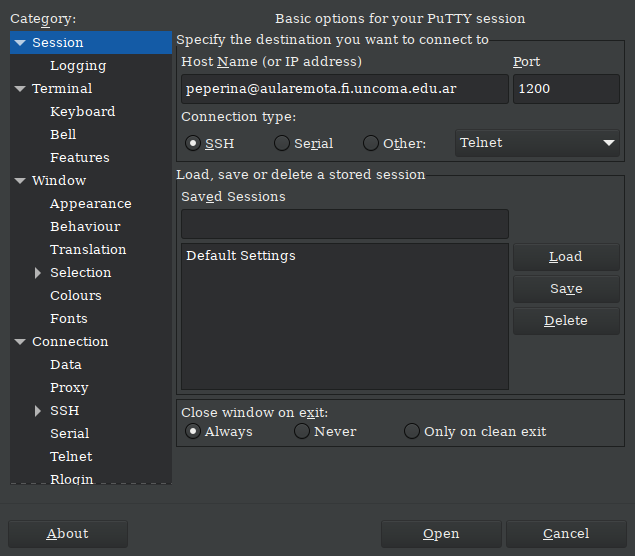
\includegraphics[width=0.75\textwidth]{img/putty.png}

    \caption{Ventana de inició y configuración de
    \emph{PuTTY}.}

    \label{imgPuTTY}

\end{figure}


    \item En el campo \emph{Host Name} ingrese su nombre de usuario seguido de
        \\cw{@aula-ssh.fi.uncoma.edu.ar}. Por ejemplo si su nombre de
        usuario es \emph{peperina}, debe ingresar
        \cw{peperina@aula-ssh.fi.uncoma.edu.ar}.

    \item En el campo \emph{Port} ingrese el número \texttt{60173}.

    \item Para no tener que re ingresar los datos cada ves que se ejecuta el
        programa, seleccione el campo \emph{Default Settings} y luego presione
        el botón \emph{Save}.

    \item Para conectarse al sistema remoto, presione el botón \emph{Open}. Se
        abrirá una terminar virtual.

    \item Ingrese su contraseña. Por cuestiones de seguridad, no se mostrará
        ningún eco de las teclas presionadas (al presionar teclas no se
        mostrarán en pantalla). Al terminar, presione la tecla 
        \emph{enter}.

    \item Si el usuario y contraseña son correctos, se iniciará el
        \emph{shell} y esperará a que ingrese un comando.

\end{enumerate}

\subsection*{\emph{SSH}}

\begin{enumerate}
    \item Abra una consola e ingrese el comando \cw{ssh -p 60173
        \emph{\$USER}@aula-ssh.fi.uncoma.edu.ar}, remplazando \emph{\$USER}
        por su usuario de los laboratorios. Presione la tecla \emph{enter}.

    \item Ingrese su contraseña. Por cuestiones de seguridad, no se mostrará
        ningún eco de las teclas presionadas (al presionar teclas no se
        mostrarán en pantalla). Al terminar, presione la tecla 
        \emph{enter}.

    \item Si el usuario y contraseña son correctos, se iniciará el
        \emph{shell} y esperará a que ingrese un comando.

\end{enumerate}

\end{document}
